\section{Uniform Robustness: Decidability at order four}
\label{section:decidability}
In this section, we prove Theorem \ref{thm:decide}. The techniques naturally apply to lower orders, and we omit their explicit treatment. Recall that we must show how to check the validity of inequality \ref{eq:crux} for all (but finitely many) $n$:
$$
\seq{\mathbf{p}, \mathbf{x_n}} \ge \max_{\mathbf{f} \in \ball}\mathbf{x_n}^T\left(\mathbf{B}^{-1}\right)^T\mathbf{f} = ||\mathbf{B}^{-1}\mathbf{x_n}|| = \sqrt{\seq{\mathbf{b_1}, \mathbf{x_n}}^2 +\dots+\seq{\mathbf{b_\kappa}, \mathbf{x_n}}^2}
$$

Our main case distinction is on the number of pairs of complex conjugates among the roots. In each case, the plan is to first decide whether a threshold index $N$ beyond which the LHS is always positive exists, and compute it. This can always be done for order four LRS \cite{joeljames3}. We then square throughout, and transfer all terms to the LHS, thus obtaining a new instance of (Ultimate) Positivity. This plan is trivial to execute when all characteristic roots are real.

Thanks to the following old result \cite[Thm. 2]{positive-dominant}, the answer to Ultimate Positivity is trivially NO if there are two pairs of complex conjugates.

\begin{proposition}[Folklore]
\label{prop:folklore}
If the characteristic polynomial has no real dominant root, then for any initialisation to the sequence, there are infinitely many positive terms, and infinitely many negative terms.
\end{proposition}

Thus, we shall concern ourselves with the case there is one pair of complex conjugate roots. Without loss of generality, we also assume that the real dominant root is $1$. 

If our LRS is \textit{simple}, i.e. it has distinct characteristic roots $1, \alpha, \gamma, \bar{\gamma}$, then decidability is rather immediate, considering the state-of-the-art. On squaring throughout after the initial Positivity check, and transferring all terms to the LHS, we get a Positivity (Problem \ref{prob:pos}) instance for a new simple LRS, this time of order at most $10$ (we get at most four roots from squaring the original roots, while there are at most six more roots from pairwise products). We assume $\alpha \ne -1$: if it were, the resulting LRS could be decomposed into two LRS of lower order, and Positivity for simple LRS is known to be decidable for order up to nine \cite{ouaknine2014positivity}. For the same reason, we can also assume $\gamma/\bar{\gamma}$ is not a root of unity: this can be efficiently detected, see Theorem \ref{thm:abelian}. Thus, the resulting LRS has at most five dominant roots, $1, \gamma, \bar{\gamma}, \gamma^2, \bar{\gamma}^2$. In this case, Positivity can be deciding for simple LRS using the techniques in \cite{ouaknine2014positivity}, regardless of the order.

The only remaining possibility, therefore, is that the characteristic roots are $1, 1, \gamma, \bar{\gamma}$. Let $0 < |\gamma| = \rho \le 1$, and we again assume that $\gamma/\bar{\gamma}$ is not a root of unity, for reasons described above. On squaring after the initial check, our LRS is of the form
\begin{align*}
&z_2n^2 + z_1n + z_0  \\
&+ x_2 n \rho^n \cos n\theta + y_2 n \rho^n \sin n\theta  \\
&+ x_1\rho^n\cos n\theta + y_1\rho^n\sin n\theta  \\
&+ x_0 \rho^{2n}\cos 2n\theta + y_0 \rho^{2n} \sin 2n\theta + w\rho^{2n} \ge 0
\end{align*}
If $\rho < 1$, the above can trivially be resolved with growth arguments, or is an easy order $3$ LRS. Thus, we assume $\rho = 1$. If $z_2 \ne 0$, then decidability is trivial; hence we assume $z_2 = 0$. In this case, our inequality can be arranged as
\begin{equation}
\label{eq:groundtruth}
{\color{red!70!black} n(z_1 + x_2\cos n\theta + y_2\sin n\theta)} + (z_0 + x_1\cos n\theta + y_1\sin n\theta + x_0\cos 2n\theta + y_0\sin 2n\theta) \ge 0
\end{equation}

Since we assume $\theta$ is not a rational approximation of $2\pi$, we can argue by Theorem \ref{thm:kronecker} (Kronecker) that $n\theta$ modulo ${2\pi}$ is dense in $[0, 2\pi]$. Define
\begin{align}
f(t) &= z_1 + x_2\cos t + y_2\sin t \\
g(t) &= z_0 + x_1\cos t + y_1\sin t + x_0\cos 2t + y_0\sin 2t
\end{align}

If $\min f(t) < 0$, then Robust Ultimate Positivity trivially does not hold; if $\min f(t) > 0$, then it can trivially be certified. Thus, we shall consider that $\min f(t) = 0$, equivalently, $z_1^2 = x_2^2 + y_2^2$. Let the minimum be attained at $\varphi$, i.e., $f(\varphi) = 0$. We have that $\varphi = \arccos(-x_2/z_1)$. Decidability is most clearly seen through a slight shift in perspective: we rotate the basis.
First, note that inequality \ref{eq:groundtruth} can easily be rewritten as (we use $t_n$ as shorthand for $n\theta - \varphi$)
\begin{equation}
\label{eq:groundtruthrewrite}
{\color{red!70!black}n(z_1 + x_2' \cos t_n)} + (z_0 + x_1'\cos t_n + y_1'\sin t_n + x_0'\cos 2t_n + y_0'\sin 2t_n) \ge 0
\end{equation}

Observe that there is nothing special about the particular representation of inequality \ref{eq:groundtruth}. The common proposition that both \ref{eq:groundtruth} and \ref{eq:groundtruthrewrite} convey is that 
$$
\left(\mathbf{e_1}^T\mathbf{A}^n\mathbf{c}\right)^2 - \left(\max_{\mathbf{d} \in \ball_{\mathbf{S}}} \mathbf{e_1}^T\mathbf{A}^n\mathbf{d}\right)^2 \ge 0
$$

On retracing our steps back to the discussion surrounding equation \ref{eq:innerprod}, we could well have chosen our basis of solutions to be $\mathbf{x_n'}\begin{bmatrix}n & 1 & \cos(n\theta - \varphi) & \sin(n\theta - \varphi) \end{bmatrix}$. This would have given us different $\mathbf{V'}, \mathbf{M'}$, and hence $\mathbf{B'}$ in equation \ref{eq:crux}, but importantly, it would generate inequality \ref{eq:groundtruthrewrite} for the same original input. We define 
\begin{align}
f_\varphi(t) &= z_1 + x_2'\cos t  \\
g_\varphi(t) &= z_0 + x_1'\cos t + y_1'\sin t + x_0'\cos 2t + y_0'\sin 2t
\end{align}
Here, $z_1 + x_2' = 0$, since the minimal $f_\varphi(0) = 0$. If $g_\varphi(0) > 0$, we are done: we can easily get a positive lower bound $f_\varphi$ for values where $g_\varphi < 0$, and get an $N$ beyond which the validity of inequality \ref{eq:groundtruthrewrite} is guaranteed. On the other hand, if $g_\varphi(0) < 0$, we argue that inequality \ref{eq:groundtruthrewrite} is violated for infinitely many $n$. Recall inequality \ref{eq:quadraticdecay}. It tells us that there are infinitely many $n$ for which $f_\varphi(n\theta + \varphi) < c/n^2$. Thus, the terms in red are infinitely often lower bounded by $c/n$, while the terms in black, for the same $n$, would be close to a negative constant. Thus, we can return NO for robust Ultimate Positivity.

The final case that remains is $g_\varphi(0) = 0$. We argue that remarkably, it does not arise at all!
\begin{lemma}
The scenario where $z_2 = 0$, $z_1 + x_2' = 0$, and $z_0 + x_1'+ x_0' = 0$ is impossible.
\end{lemma}
\begin{proof}
Suppose that $\mathbf{b_1}^T, \dots, \mathbf{b_4}^T$ are the rows of the matrix $(\mathbf{B'})^{-1}$, and $\mathbf{u_1}, \dots, \mathbf{u_4}$ are the columns. Our inequality is:
\begin{align*}
(p_1 n + p_2 + p_3\cos(n\theta - \varphi) + p_4\sin(n\theta - \varphi))^2 \\
- \left( \dots + (b_{i1} n + b_{i2} + b_{i3}\cos(n\theta - \varphi) + b_{i4}\sin(n\theta - \varphi))^2 + \dots \right) \ge 0
\end{align*}
In the table, we explicitly give each coefficient of inequality \ref{eq:groundtruthrewrite}.
\begin{table}[H]
\begin{tabular}{|l|l|l|}
  \hline
   \textbf{Term}& \textbf{Coefficient}& {\bf Explicitly} \\
  \hline
  $n^2$ & $z_2 = 0$ & $p_1^2 - \seq{\mathbf{u_1}, \mathbf{u_1}}$ \\
   \hline
  $n$ & $z_1$ & $2p_1p_2 - 2\seq{\mathbf{u_1}, \mathbf{u_2}}$ \\
   \hline
  $n\cos (n\theta - \varphi)$ & $x_2'$ & $2p_1p_3 - 2\seq{\mathbf{u_1}, \mathbf{u_3}}$ \\
   \hline
  $n\sin (n\theta - \varphi)$ & $y_2' = 0$ & $2p_1p_4 - 2\seq{\mathbf{u_1}, \mathbf{u_4}}$ \\
   \hline
  $1$ & $z_0$ & $p_2^2 + \frac{1}{2}(p_3^2 + p_4^2) - \seq{\mathbf{u_2}, \mathbf{u_2}} - \frac{1}{2}
 (\seq{\mathbf{u_3}, \mathbf{u_3}} + \seq{\mathbf{u_4}, \mathbf{u_4}})$ \\
  \hline
  $\cos (n\theta-\varphi)$ & $x_1'$ & $2p_2p_3 - 2\seq{\mathbf{u_2}, \mathbf{u_3}}$ \\
   \hline
  $\sin (n\theta-\varphi)$ & $y_1'$ & $2p_2p_4 - 2\seq{\mathbf{u_2}, \mathbf{u_4}}$ \\
   \hline
  $\cos (2n\theta - 2\varphi)$ & $x_0'$ & $\frac{1}{2}(p_3^2 - p_4^2) - \frac{1}{2}(\seq{\mathbf{u_3}, \mathbf{u_3}} - \seq{\mathbf{u_4}, \mathbf{u_4}})$ \\
   \hline
  $\sin (2n\theta - 2\varphi)$ & $y_0'$ & $2p_3p_4 - 2\seq{\mathbf{u_3}, \mathbf{u_4}}$ \\
  \hline
\end{tabular}
\end{table}
Suppose, for the sake of contradiction, the scenario actually occurs. We then respectively have
\begin{align*}
p_1^2 &= \seq{\mathbf{u_1}, \mathbf{u_1}} \\
p_1(p_2 + p_3) &= \seq{\mathbf{u_1}, \mathbf{u_2} + \mathbf{u_3}} \\
(p_2 + p_3)^2 &= \seq{\mathbf{u_2} + \mathbf{u_3}, \mathbf{u_2} + \mathbf{u_3}}
\end{align*}
This implies that $|\seq{\mathbf{u_1}, \mathbf{u_2} + \mathbf{u_3}}| = ||\mathbf{u_1}||\cdot||\mathbf{u_2} + \mathbf{u_3}||$, i.e. $\mathbf{u_1}$ is a scaled multiple of $\mathbf{u_2} + \mathbf{u_3}$. This contradicts the fact that the columns of the invertible $(\mathbf{B'})^{-1}$ are linearly independent, and we're done.
\end{proof}

\section{Non-uniform Robustness: Decidability at order five}
\label{section:decidability2}
In this section, we deploy sophisticated mathematical arsenal to prove Theorem \ref{thm:decide2}. As before, the techniques naturally apply to lower orders, and we omit their explicit treatment. Recall equation \ref{eq:grouping} and the surrounding discussion:
\begin{equation}
u_n/n^d\rho^n = \begin{bmatrix}
{\color{red!70!black} \mathbf{q}_{dom}^T(n) } & \mathbf{q}_{res}^T(n)
\end{bmatrix}
\begin{bmatrix}
{\color{red!70!black} \mathbf{p}_{dom}} \\
\mathbf{p}_{res}
\end{bmatrix}
\end{equation}
The crucial first task is to check whether for all points $\mathbf{p'}$ in the neighbourhood, \\$\liminf_{n\in\naturals}\seq{\mathbf{q}_{dom}(n), \mathbf{p'}_{dom}} = \mu(\mathbf{p'}) \ge 0$. For an arbitrary point $\mathbf{p'}$, the high-level approach to do this is to:

\begin{enumerate}
\item Replace $\mathbf{q}_{dom}$ by $\mathbf{g}(\boldsymbol{\phi})$, such that $\mathbf{q}_{dom}(n) = \mathbf{g}(n\boldsymbol{\theta})$. Find a set $T$ that $n\boldsymbol\theta$ are dense in. (Masser, Theorem \ref{thm:abelian}, and Kronecker, Theorem \ref{thm:kronecker})
\item Argue that $\liminf_n  \seq{\mathbf{q}_{dom}(n), \mathbf{p'}_{dom}} = \min_{\boldsymbol{\phi} \in T} \seq{\mathbf{g}(\boldsymbol{\phi}), \mathbf{p'}_{dom}}  = \mu(\mathbf{p'})$
\item Query $\mu$. Let $\psi(\mathbf{p'})$ denote the formula that $\mu(\mathbf{p'}) \ge 0$ (First Order Theory of Reals, Renegar, Theroem \ref{thm:renegar})
\end{enumerate}
The first task then reduces to evaluating the truth of the sentence 
$$
\forall \mathbf{p'}.~ (\mathbf{p'} - \mathbf{p})^T\mathbf{M}(\mathbf{p'} - \mathbf{p}) \le 1 \Rightarrow \psi(\mathbf{p'})
$$
The neighbourhood may intersect the critical region where $\mu = 0$. If there are no non-dominant terms, this is irrelevant; but otherwise decidability hinges on whether we can handle the intersection. Geometric arguments, and the underlying decidability of the non-robust problems at low orders \cite{joeljames3} give us our decidability results.

\subsection{Mathematical tools}
\label{arsenal}
The first step of our plan was to replace the discrete $\mathbf{q}_{dom}$, by $\mathbf{g}$, parametrised by $\boldsymbol\phi$ that come from a continuous set $T$. The preliminary step is to efficiently elicit additive relations among $\boldsymbol\theta$, which translate into multiplicative relationships among the corresponding characteristic roots $e^{i\boldsymbol\theta}$.
 \begin{theorem}[Masser \cite{Masser}]
  \label{thm:abelian}
  Let $e^{i \theta_1},...,e^{i \theta_k}$ be complex algebraic numbers of unit modulus. Consider the free abelian group $L$ defined by $L = \{(\lambda_1, \ldots ,\lambda_k) \in \mathbb{Z}^k: 
  e^{i (\lambda_1 \theta_1 + \cdots +  \lambda_k \theta_k)} = 1 \}$. 
  The group $L$ has a finite generator set $\{ \mathbf{l_1}, \ldots, \mathbf{l_p}\} \subset \mathbb{Z}^k$ with $p \le k$. The generator set can be computed in time polynomial and
  each entry in the generator set is polynomially bounded in the sizes of the representations of $e^{i \theta_1},...,e^{i \theta_k}$.
  \end{theorem}
 Given $e^{2i\theta}$, if an $n$ such that $e^{2i n \theta} = 1$ exists ($\theta$ is a rational multiple of $2\pi$), this $n$ is bounded, and can be efficiently found by enumeration. Similarly, one can check whether $\alpha^n = \beta$ (is $n\theta - \varphi$ ever an integer multiple of $2\pi$?). 
 
Let $T$ be the set of all $\boldsymbol\phi$ such that for all $\mathbf{l} \in L$ above, $\seq{\mathbf{l}, \boldsymbol\phi} \in 2\pi\integers$. Kronecker's theorem on simultaneous Diophantine approximation, as strengthened by \cite{joeljames3, ouaknine2014positivity}, directly establishes that $n\boldsymbol\theta$ are dense in $T$.
 
 \begin{theorem}[Kronecker \cite{Kronecker}]
  \label{thm:kronecker}
  Let $\theta_1, ... , \theta_k, \phi_1, ... , \phi_k \in [0, 2\pi)$. Then the following are equivalent:
  \begin{enumerate}
\item For every tuple $(\lambda_1,...\lambda_k)$ of integers with 
    $\lambda_1 \theta_1 + \cdots +  \lambda_k \theta_k \in 2\pi\integers$, 
  we have \\$\lambda_1 \phi_1 + \cdots + \lambda_k \phi_k \in 2\pi\integers$.
  \item For any $\epsilon > 0$, there exists an arbitrarily large $n$ such that for all 
    $1 \le j \le k$ we have $| n \theta_j - \phi_j| \le \epsilon$.
    \end{enumerate}
  \end{theorem}
  
Since $\mathbf{q}_{dom}(n) = \mathbf{g}(n\boldsymbol{\theta})$, this immediately implies that for all $\mathbf{p'}$
\begin{equation}
\liminf_n  \seq{\mathbf{q}_{dom}(n), \mathbf{p'}_{dom}} = \min_{\boldsymbol{\phi} \in T} \seq{\mathbf{g}(\boldsymbol{\phi}), \mathbf{p'}_{dom}}  = \mu(\mathbf{p'})
\end{equation}

We now turn to computing $\mu$. Fortunately, $F$ is multilinear, and, given $\mathbf{p}$, all the constants involved are algebraic. Thus, we can use the First Order Theory of the Reals. Let $\sigma(a_1, a_2, b)$ denote $a_1^2 + a_2^2 = 1 \land b^2 =1$. Then, $\mu$ is the unique satisfying assignment of the following formula $\chi(\mu)$
$$
(\forall a_1, a_2, b.~ \sigma(a_1, a_2, b) \implies F(\mathbf{p}, a_1, a_2, b) \ge \mu) \land (\exists a_1, a_2, b.~ \sigma(a_1, a_2, b) \land F(\mathbf{p}, a_1, a_2, b) = \mu)
$$
Renegar's Theorem (Theorem \ref{thm:renegar}) asserts that this algebraic $\mu$ can be computed via quantifier elimination. Finally, we note that when $\theta$ is not a rational multiple of $2\pi$, the minimum of $1 - \cos(n\theta - \varphi)$ is attained at most once: we can use Theorem \ref{thm:abelian} to check if this is the case. In fact, we can provide a threshold $N_1$ beyond which $n\theta \ne \varphi$. 



If there are no residual terms, we are already done at this point. In the event residual terms have non-zero contribution, decidability hinges on whether we can handle points where $\mu = 0$. If there are two pairs of complex conjugates among the dominant roots, then all five terms are dominant (recall Proposition \ref{prop:folklore}!)

\begin{figure}[h]

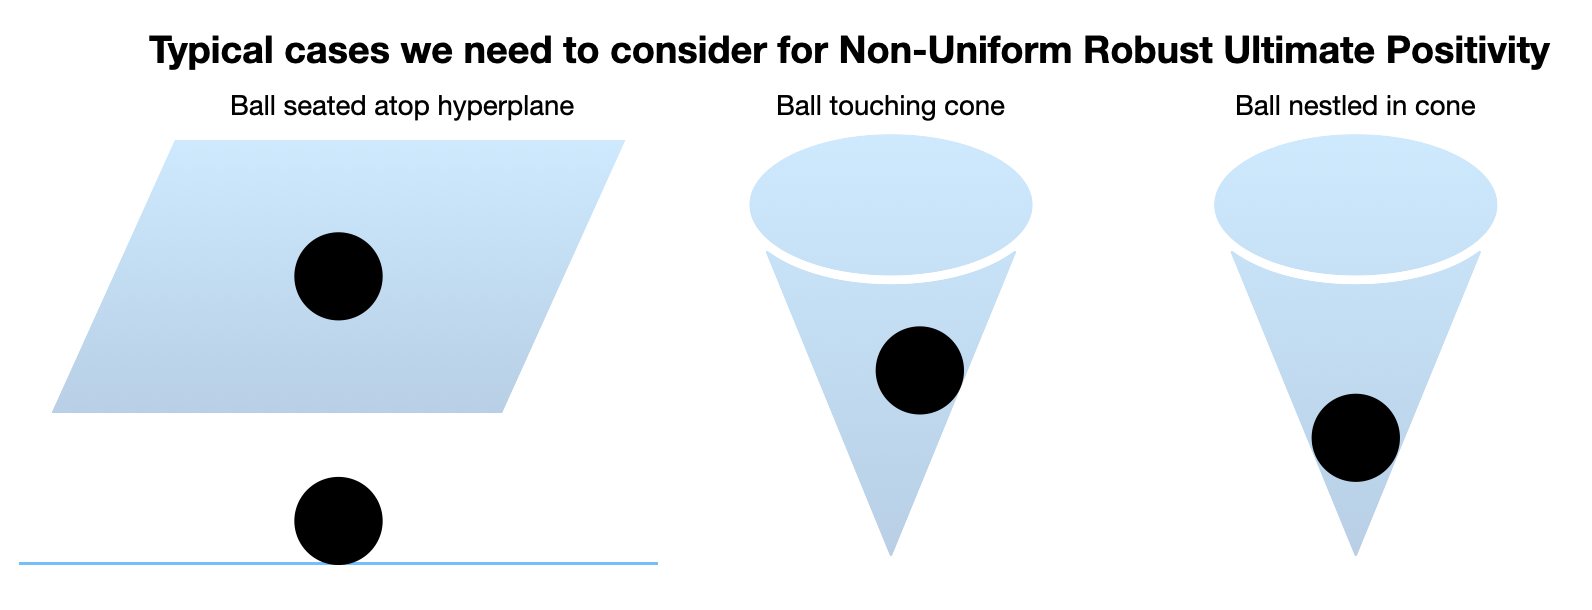
\includegraphics[width=\textwidth]{picture1.png}
\caption{Visual intuition}
\label{fig:geometricpicture}
\end{figure}

Hence, we consider that there is at most one complex conjugate pair among the dominant roots. This requires slightly more insight of the geometrical nature of the solution set of $\psi_0$ (Figure \ref{fig:geometricpicture}). See \cite{originalstacs,originalarxiv} for an exposition of the geometric intuition. If there are just one or two dominant terms, they are necessarily real. The region $\mu(\mathbf{p}) = 0$ will simply be the union of at most two hyperplanes. ($z = 0$, or $z - |w| = 0$). Here, the intersection of the ball with $\mu = 0$ consists of at most two points. Since Ultimate Positivity is decidable up to order $5$ \cite{joeljames3}, it can explicitly be checked.

Finally, let there be one pair of complex conjugates $e^{\pm i\theta}$ among the dominant roots. It is clear that if $\theta$ is a rational multiple of $2\pi$, $\mu = 0$ will be a union of finitely many hyperplanes (of the form $z - |w| - x\cos \theta_0 - y\sin \theta_0 = 0$). Here again, the finite intersection can be explicitly checked. In the case when $e^{i\theta}$ is not a root of unity, we recall equation \ref{eq:cone}: the set of $\mathbf{p}$ for which $\mu = 0$ is given by
\begin{equation}
z - |w| - \sqrt{x^2 + y^2} = 0
\end{equation}
In this case, it is a union of \textit{infinitely} many hyperplanes of the form $z - |w| - x \cos \phi - y\sin \phi = 0$. As established by the validity of equation \ref{eq:firsttask}, the centre of the neighbourhood is distance at least $r$ away from each of these hyperplanes. If the surface of the $r$-ball touches any of these hyperplanes, the point must be obtained by traversing along the normal from the centre. Thus, the point must be $(z_0 - \frac{r}{\sqrt{3}}, w_0 \pm \frac{r}{\sqrt{3}}, x_0 + \frac{r}{\sqrt{3}}\cos\phi, y_0 +  \frac{r}{\sqrt{3}}\sin\phi, v_0)$. Note that the residual coordinate is unchanged! Substituting this into the hyperplane equation gives us a quadratic equation in $\cos \phi$: this holds for zero, one, two, or all $\phi$. We already know how to handle a finite intersection.

If this holds for all $\phi$, then we use Theorem \ref{thm:kronecker} (Kronecker's density) to argue that for every $n$, there exists a point on the surface of the ball such that the dominant contribution is zero. As observed, the residual part is the same as the centre for such points. Thus, in this case, it is entirely up to the residual terms of the centre to guarantee Robust Ultimate Positivity. This is a decidable instance of regular Ultimate Positivity at lower order, and we are done.
